\documentclass[11pt,spanish,a4paper]{article}

% Versión 1.er cuat 2021 Víctor Bettachini < vbettachini@unlam.edu.ar >

\usepackage[T1]{fontenc}
\usepackage[utf8]{inputenc}

\usepackage[spanish, es-tabla]{babel}
% \def\spanishoptions{argentina} % Was macht dass?
% \usepackage{babelbib}
% \selectbiblanguage{spanish}
% \addto\shorthandsspanish{\spanishdeactivate{~<>}}


\usepackage{graphicx}
\graphicspath{{./figuras/}{../LaTeX/}{../figurasLaTeX/}}
% \usepackage{float}

\usepackage[arrowdel]{physics}
\newcommand{\pvec}[1]{\vec{#1}\mkern2mu\vphantom{#1}}
% \usepackage{units}
\usepackage[separate-uncertainty= true, multi-part-units= single, range-units= single, range-phrase= {~a~}, locale= FR]{siunitx}
\usepackage{isotope} % $\isotope[A][Z]{X}\to\isotope[A-4][Z-2]{Y}+\isotope[4][2]{\alpha}

\usepackage{tasks}
\usepackage[inline]{enumitem}
% \usepackage{enumerate}

\usepackage{hyperref}

% \usepackage{amsmath}
% \usepackage{amstext}
% \usepackage{amssymb}

\usepackage{tikz}
\usepackage{tikz-3dplot}
\usepackage{tikz-dimline}
\usetikzlibrary{calc}
% \usetikzlibrary{math}
\usetikzlibrary{arrows.meta}
\usetikzlibrary{snakes}
\usetikzlibrary{decorations}
\usetikzlibrary{decorations.pathmorphing}
\usetikzlibrary{patterns}

\usepackage[hmargin=1cm,vmargin=3cm, top= 0.75cm,nohead]{geometry}

\usepackage{lastpage}
\usepackage{fancyhdr}
\pagestyle{fancyplain}
\fancyhf{}
\setlength\headheight{28.7pt} 
\fancyhead[LE, LO]{\textbf{Mecánica Analítica Computacional} }
% \fancyhead[LE, LO]{\textbf{Mecánica General} }
\fancyhead[RE, RO]{\href{https://ingenieria.unlam.edu.ar/}{$\vcenter{\hbox{
\includegraphics[height=1cm]{ambos.pdf}}}$}}
\fancyfoot{\href{https://creativecommons.org/licenses/by-nc-sa/4.0/deed.es_ES}{$\vcenter{\hbox{
\includegraphics[height=0.4cm]{by-nc-sa_80x15.pdf}}}$} \href{https://ingenieria.unlam.edu.ar/}{DIIT - UNLaM}}
\fancyfoot[C]{ {\tiny Actualizado al \today} }
\fancyfoot[RO, LE]{Pág. \thepage/\pageref{LastPage}}
\renewcommand{\headrulewidth}{0pt}
\renewcommand{\footrulewidth}{0pt}



\begin{document}
\begin{center}
  \textsc{\large Mecánica general}\\
  \textsc{\large Coordenadas generalizadas | Lagrangiano}
\end{center}

\noindent
%De poder resolver estos problemas en forma autónoma puede asumir que adquirió los conocimientos mínimos sobre los temas abordados en la semana.
%No dude en consultar a docentes y compañeros si no puede terminarlos.
Los problemas marcados con (*) tienen alguna dificultad adicional, no dude en consultar.
\begin{enumerate}


\item Escriba y resuelva la ecuación que describe la dinámica de un péndulo de longitud $l$ en presencia de un campo gravitatorio de constante $g$. Discuta todas las aproximaciones que realiza.



\item \begin{minipage}[t][3.5cm]{0.7\textwidth}
\textbf{Landau \S5 ej. 2}
Escriba el Lagrangiano en función de las coordenadas generalizadas sugeridas por las figura para un péndulo oscilando en un plano de masa \(m_2\) cuyo punto de suspensión, de masa \(m_1\), puede desplazarse sobre una recta horizontal.

Verifique que recupera el Lagrangiano de un péndulo simple de asumir fija la masa \(m_1\).
\end{minipage}
	\begin{minipage}[c][1cm][t]{0.3\textwidth}
        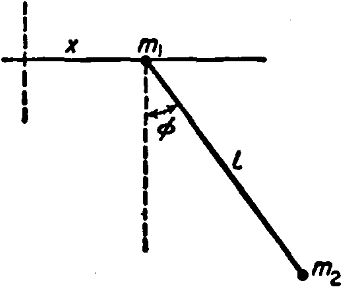
\includegraphics[width=0.75\textwidth]{landauS52_fig2.png}
\end{minipage}




\item \begin{minipage}[t][4.5cm]{0.7\textwidth}
\textbf{Landau \S5 ej. 1}
Escriba el Lagrangiano para un péndulo doble oscilando en un plano en función de las coordenadas generalizadas sugeridas por las figura.

Ayuda: \( \cos{\alpha \pm \beta }=\cos{ \alpha} \cos{ \beta \mp \sin \alpha} \sin{ \beta } \)

Verifique que recupera el Lagrangiano de un péndulo simple de asumir \(m_1=0\), \(\varphi_1 = \varphi_2 = \varphi\) y \(l_1 = l_2 = \frac{l}{2}\).
\end{minipage}
	\begin{minipage}[c][2.5cm][t]{0.3\textwidth}
	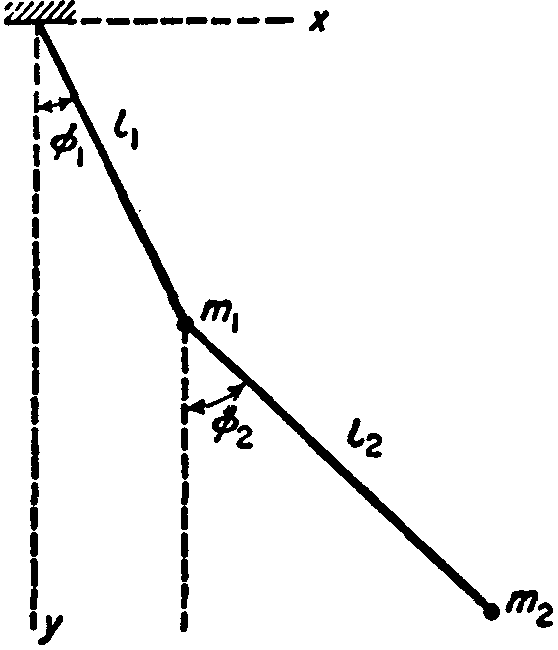
\includegraphics[width=0.75\textwidth]{landauS52_fig1.png}
\end{minipage}



\item \begin{minipage}[t][4.5cm]{0.7\textwidth}
(*) \textbf{Landau \S5 ej. 3}
Calcular el Lagrangiano para un péndulo plano cuyo punto de suspensión se desplaza  en un círculo vertical de radio \(a\) a través:
\begin{enumerate}
\item de su circunferencia con una frecuencia \(\gamma\),
\item de su diámetro horizontal según \(a \cos{(\gamma t)}\),
\item de su  diámetro vertical según \(a \cos{(\gamma t)}\).
\end{enumerate}
\end{minipage}
	\begin{minipage}[c][2.5cm][t]{0.3\textwidth}
	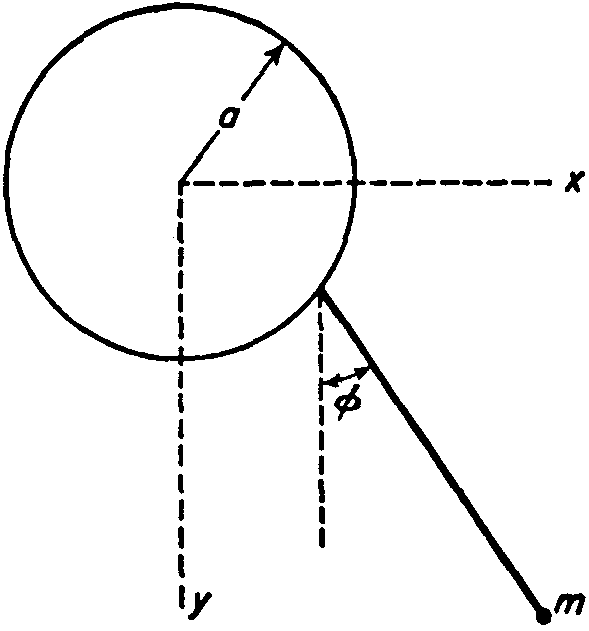
\includegraphics[width=0.75\textwidth]{landauS52_fig3.png}
\end{minipage}



\item \begin{minipage}[t][4.5cm]{0.7\textwidth}
(*) \textbf{Landau \S5 ej. 4}
	Calcular el Lagrangiano para el sistema de figura donde la partícula con \(m_2\) se desplaza sobre un eje vertical, y todo el sistema gira con una velocidad angular constante \(\Omega\) en torno a ese eje.
\end{minipage}
	\begin{minipage}[c][2.5cm][t]{0.3\textwidth}
	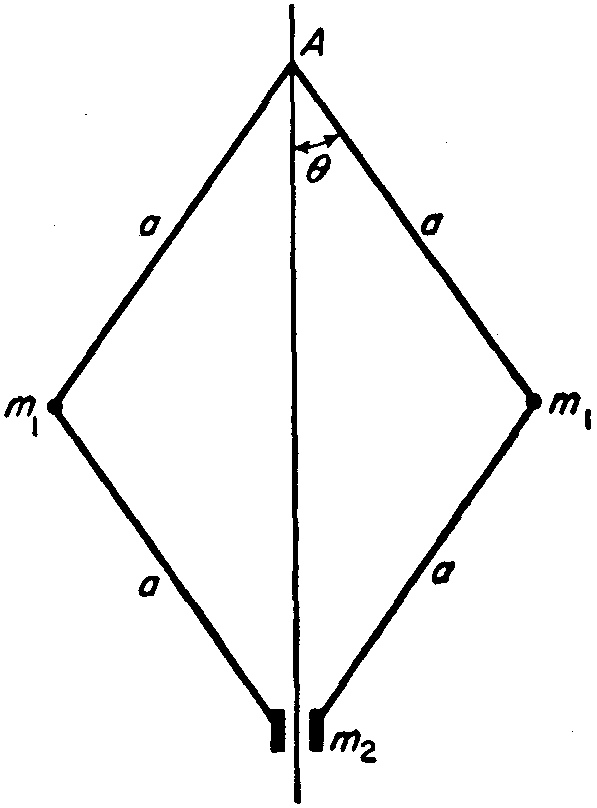
\includegraphics[width=0.75\textwidth]{landauS52_fig4.png}
\end{minipage}



\end{enumerate}
\end{document}
